\chapter{Context of the work}
\minitoc
\newpage

\setcounter{secnumdepth}{0} % Set the section counter to 0 so next section is not counted in toc
% ----------------------- Introduction ----------------------- %
\section{Introduction}
This chapter outlines the framework of our project, providing a comprehensive overview of the host organization, project goals, and the challenges we aim to address. It sets the stage for a comparative analysis of existing methodologies, leading to the selection of an optimized strategy for successful project execution. Our objective is to delve into the project’s environment, offering nuanced insights into its significance for the hosting entity and the industry at large.

\setcounter{secnumdepth}{2} % Resume counting the sections for the toc with a depth of 2 (Sections and sub-sections)
% ----------------------------------- SECTIONS (v) ----------------------------------- %
% ----------------------- General framework of the internship ----------------------- %
\section{Host Organization Profile: Incedo Services GmbH}
Incedo Services GmbH specializes in driving the digital transformation of small to medium-sized businesses through its expertise in IT consulting, custom software development, and ERP consulting services. With proprietary tools such as Haufe X360, Activewhere, and the Incedo Lead Generator at its disposal, Incedo is dedicated to delivering tailored solutions that foster business growth and enhance operational efficiency. The company’s foundation is built on a commitment to innovation and customer satisfaction, positioning Incedo as a reliable partner for overcoming the challenges of digital transition.


\begin{figure}[h]
    \centering
    
\includegraphics[width=5cm]{src/assets/chapters/incedo-logo.png} 
    \caption{Incedo Logo}
    \label{fig:incedo-logo}
  \end{figure}


  \begin{table}[H]
    \centering
    \begin{tabular}{|p{4cm}|p{9cm}|}
      \hline
      \textbf{Services} & 
      \begin{itemize}
        \item \textbf{IT Consulting:}
        \begin{itemize}
          \item Providing tailored consulting to optimize IT infrastructure and software solutions for businesses.
        \end{itemize}
        \item \textbf{Software Development:}
        \begin{itemize}
          \item Developing custom software solutions tailored to the specific needs of clients, enhancing business innovation and efficiency.
        \end{itemize}
        \item \textbf{ERP Consulting:}
        \begin{itemize}
          \item Expert advice on ERP system implementation and optimization, with a deep understanding of business processes.
        \end{itemize}
        \item \textbf{Proprietary Products:}
        \begin{itemize}
          \item \textbf{Haufe X360 \& Activewhere:}
          \begin{itemize}
            \item Specialized products designed to assist businesses in various operational aspects.
          \end{itemize}
          \item \textbf{Incedo Lead Generator:}
          \begin{itemize}
            \item A tool for optimizing outreach campaigns and generating high-quality leads.
          \end{itemize}
        \end{itemize}
      \end{itemize}
      \\
      \hline
      \textbf{Phone number} & +49 711 674300 \\
      \hline
      \textbf{Address} & Leuschnerstraße 44, 70176 Stuttgart, Germany \\
      \hline
      \textbf{Website} & \url{https://incedo.de/en/} \\
      \hline
    \end{tabular}
    \caption{Incedo Services Information}
    \label{tab:incedo-services}
  \end{table}
  
 
\section{Project Overview}
Aermax is a company that specializes in offering services at altitudes specifically focusing on tasks that demand precision, safety, and expertise. These services play a role in ensuring the durability and long-term viability of buildings. They encompass a range of activities such as:
\begin{itemize}
    \item Cleaning of Elevated Structures: This involves the removal of dirt, debris, and other materials from high surfaces, using specialized equipment and techniques to ensure thorough cleaning without compromising safety.
    \item Rope Access Solutions: AerMax offers solutions for accessing hard-to-reach areas, employing advanced rope access techniques that enable efficient and safe completion of tasks.
    \item Roof Repairs: The company conducts repairs on roofs to address damages and wear, ensuring the building remains structurally sound and protected from environmental elements.
  \end{itemize}

  In the realm of operational excellence, Aermax distinguishes itself through:

  \begin{itemize}
    \item Innovative Service Platform: An advanced digital ecosystem designed to streamline the management of projects and tasks. This platform offers features like:
    \begin{itemize}
      \item Transparent Workflow: Ensuring a clear and cohesive process from project inception to completion, facilitating seamless collaboration between teams.
      \item Real-Time Updates: Providing stakeholders with immediate information on progress, enhancing communication, and building trust.
    \end{itemize}
  \end{itemize}
  
  After releasing the version of the Aermax platform, our team is dedicated to making valuable contributions to this project. We plan on incorporating features and resolving any existing issues to enhance the performance of the platform. This next phase aims to improve user experience, increase functionality, and tackle the challenges that were identified during its rollout. Our primary goal is to improve and ensure that the Aermax service platform remains a leader in managing high-altitude services.
    
\subsection{Problem Assessment and Challenges}
Upon evaluating Aermax Company's structure, for handling high-altitude service projects it has come to light that there are significant shortcomings in the current management system. These gaps present hurdles that require an examination and strategic revamping. One prominent challenge revolves around the lack of clarity regarding worker allocation and task management. In other words, the company struggles to determine which workers are assigned to specific tasks at any given moment resulting in inefficiencies and potential safety hazards, in the ever-changing conditions characteristic of high-altitude environments.

Identified Issues:
\begin{itemize}[leftmargin=*]
  \item Lack of Worker-Task Visibility: AerMax currently needs to work on a system that provides clear, real-time insights into worker locations, assigned tasks, and progress reports. This opacity complicates project management and hampers the ability to respond swiftly to changes or emergencies.
  \item Inadequate Task Allocation: The process for assigning tasks to workers is not optimized for the specific demands and skill sets required for high-altitude projects. This can result in mismatches between worker capabilities and project needs, affecting both safety and productivity.
  \item Communication Gaps: Effective communication is crucial for the success of high-altitude projects, yet current mechanisms are insufficient for the seamless exchange of information between workers and management. This leads to delays, misunderstandings, and increased risk.
  \item Compliance and Documentation: Ensuring compliance with industry standards and maintaining accurate documentation presents another layer of complexity. The current system lacks the efficiency to manage these aspects effectively, risking non-compliance and potential legal issues.
  \item Worker Well-being: The physical and mental well-being of workers is paramount, yet there is a need for a more structured approach to monitoring health, providing support, and ensuring the overall safety of the workforce in challenging environments.
\end{itemize}

These identified issues underscore the necessity for AerMax to develop an innovative platform. Such a platform must not only address these specific challenges but also offer a holistic solution that enhances safety, efficiency, and worker satisfaction through improved task allocation, real-time visibility, seamless communication, and compliance tracking.

 

\subsection{Competitor Benchmarking}
\subsubsection*{\underline{Competitors Selection}}
In our investigation of existing solutions, we meticulously assessed various platforms and pinpointed four that most closely meet our specific requirements. We will provide a summary of these selected solutions, emphasizing their main features and functionalities.

\subsubsection*{I.4.1 Competitors Selection}
\addcontentsline{toc}{subsubsection}{I.4.1 Competitors Selection}
In our investigation of existing solutions, we meticulously assessed various platforms and pinpointed four that most closely meet our specific requirements. We will provide a summary of these selected solutions, emphasizing their main features and functionalities.

\subsubsection*{I.4.1.1 Blauarbeit}
\addcontentsline{toc}{subsubsection}{\hspace{1.5em}I.4.1.1 Blauarbeit}
 
Blauarbeit is an online platform where German citizens can look for experts to help with hard and sometimes dangerous tasks like structure and fixing effects in their homes or workplaces. It's like a big directory filled with experts who are good at fixing effects like broken pipes, electrical problems, or erecting new structures. This makes it easy for anyone to find the right person for the job without having to search all over the place. Plus, Blauarbeit makes sure that all the workers are dependable and secure, so people can feel confident about hiring them. Whether it's repairing a dense roof or cleaning at a high altitude and dangerous place.

\begin{figure}[H]
    \centering
    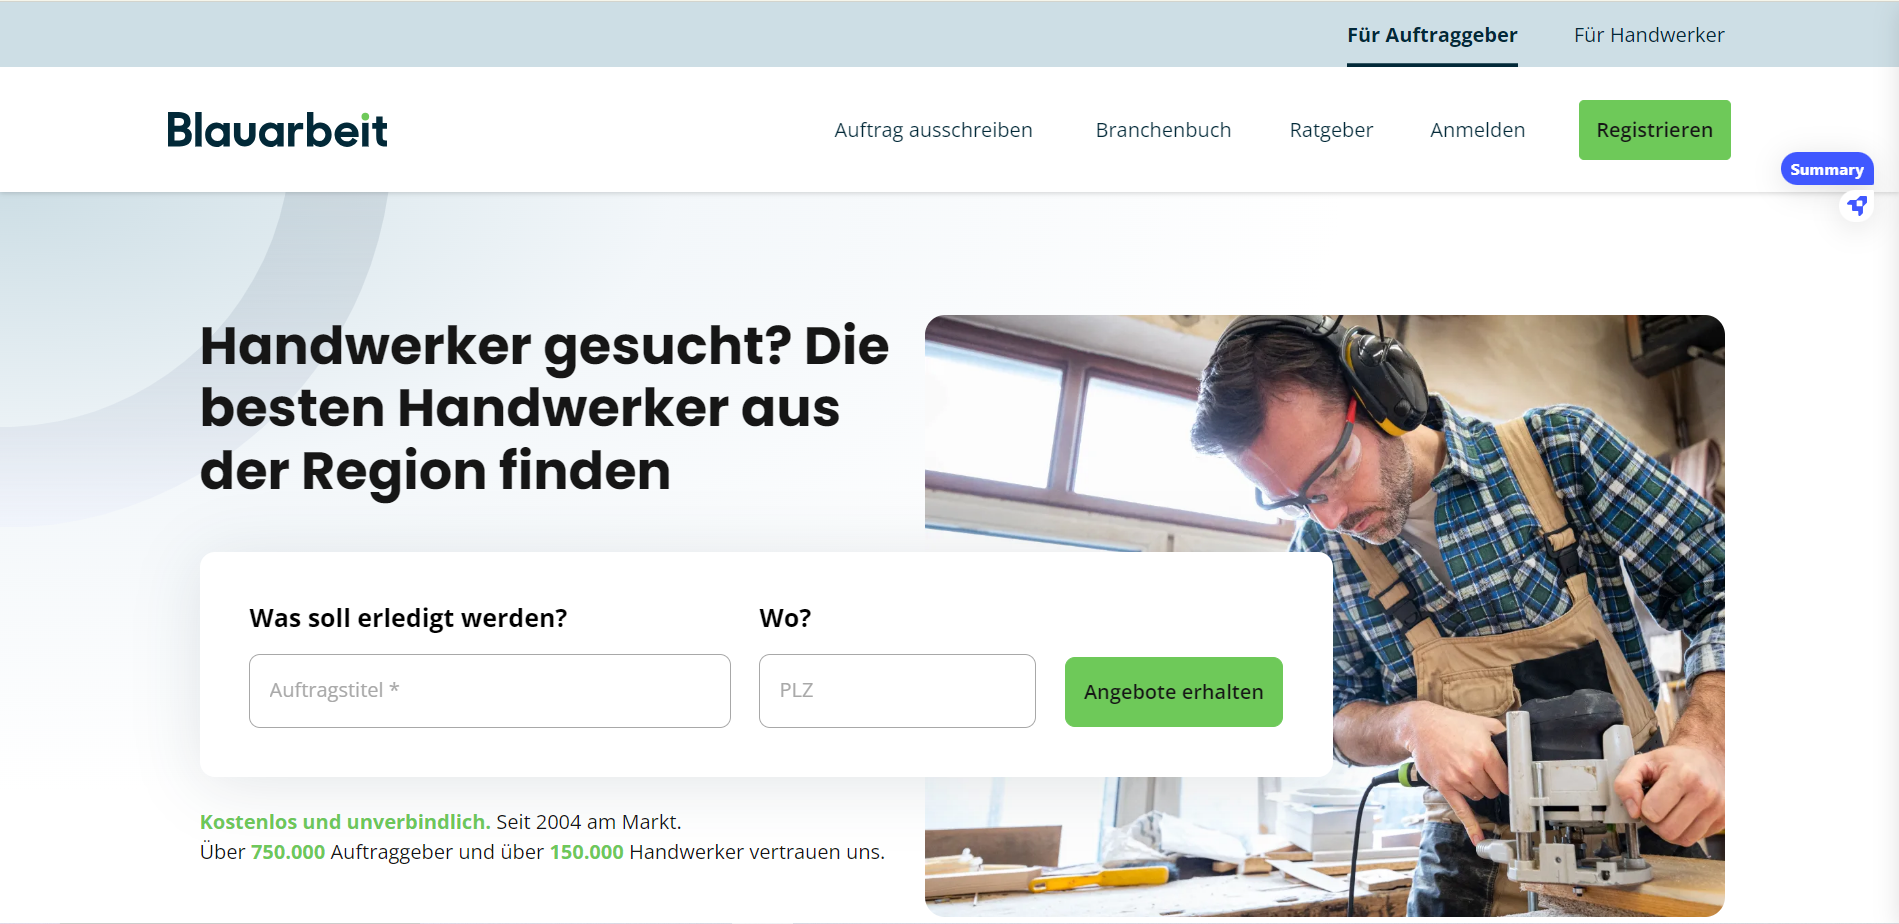
\includegraphics[width=1\textwidth]{src/assets/chapters/Blaurabeit.PNG}
    \caption{Blaurabeit Homepage}
    \label{fig:blaurabeit_image}
\end{figure}

\subsubsection*{I.4.1.2 IRATA Hub}
\addcontentsline{toc}{subsubsection}{\hspace{1.5em}I.4.1.2 IRATA Hub}

IRATA Hub is a specialized digital platform catering to the unique needs of companies and technicians engaged in industrial rope access projects. Offering a range of functionalities, it simplifies project management while ensuring adherence to industry standards. From managing certification records and tracking training courses to scheduling equipment inspections and centralizing project documentation, IRATA Hub streamlines administrative tasks with efficiency. Moreover, it promotes safety by providing technicians with up-to-date safety procedures and facilitating real-time communication among project teams. With its comprehensive features, IRATA Hub serves as a valuable tool for enhancing project management and safety in industrial rope access projects.


\subsubsection*{I.4.1.3 Fieldwire}
\addcontentsline{toc}{subsubsection}{\hspace{1.5em}I.4.1.3 Fieldwire}

Fieldwire is a robust project management software designed for construction teams to streamline collaboration and task management. Its key functionalities include task management, plan viewing, issue tracking, and real-time communication. With Fieldwire, users can create and assign tasks, upload and view construction plans, document issues and observations, and communicate with team members instantly. The platform facilitates seamless coordination among team members, allowing for efficient project planning and execution. By centralizing project information and communication, Fieldwire helps construction teams stay organized, ensure project accuracy, and meet project deadlines effectively.

\begin{figure}[H]
    \centering
    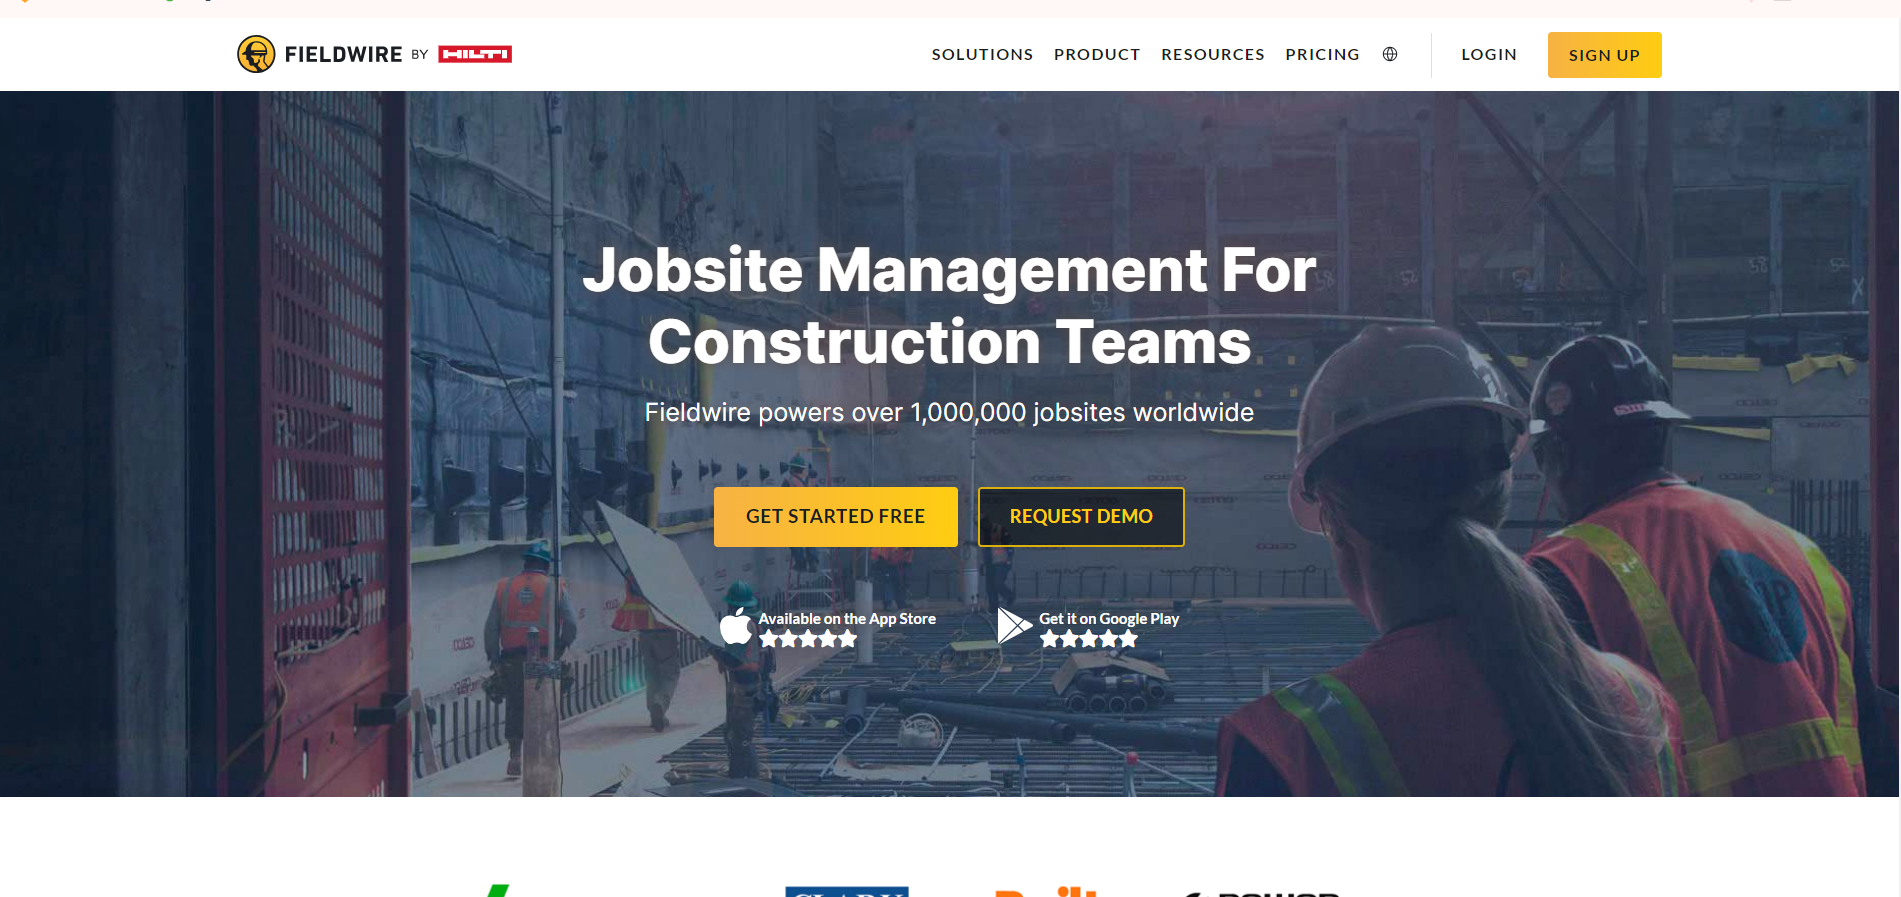
\includegraphics[width=1\textwidth]{src/assets/chapters/fieldwire.PNG}
    \caption{Fieldwire Homepage}
    \label{fig:fieldwire_image}
\end{figure}
 
\subsubsection*{I.4.1.4 MyHammer}
\addcontentsline{toc}{subsubsection}{\hspace{1.5em}I.4.1.4 MyHammer}

MyHammer is an online platform based in Germany that connects homeowners and businesses with local tradesmen and service providers for various construction, renovation, and repair projects.
MyHammer provides various features including a wide range of services, a transparent bidding process, a mobile-friendly interface


\begin{figure}[H]
    \centering
    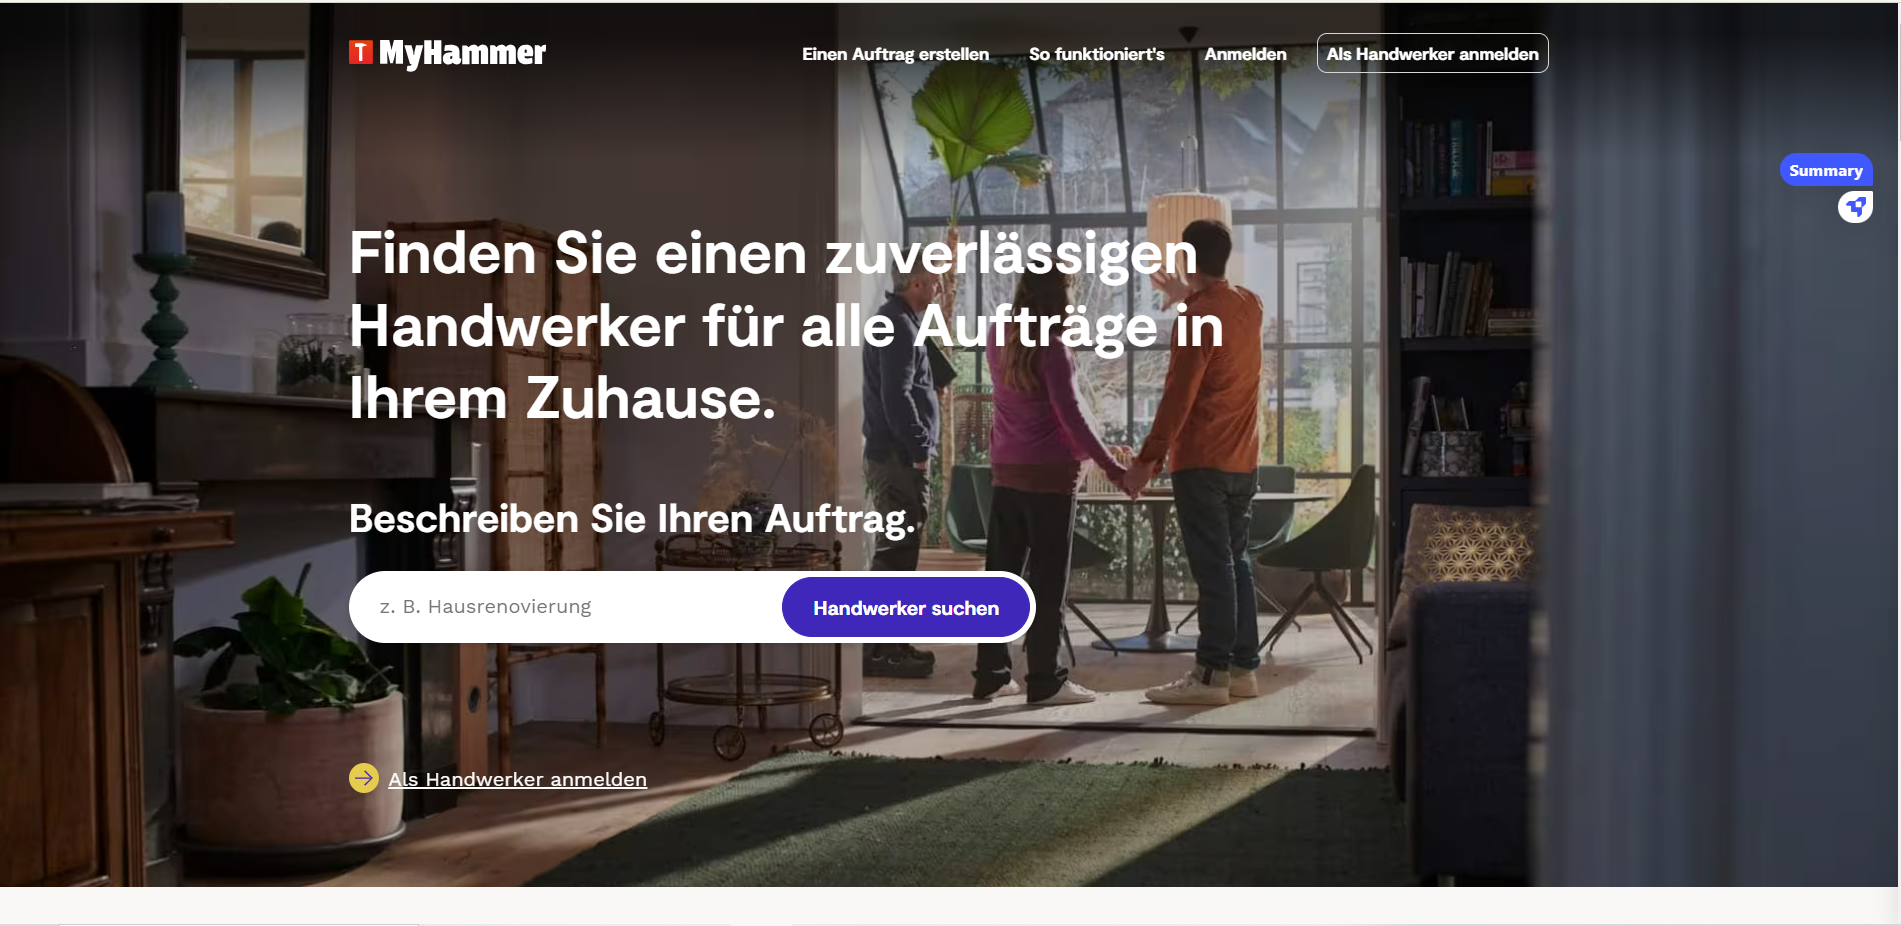
\includegraphics[width=1\textwidth]{src/assets/chapters/myHammer.PNG}
    \caption{MyHammer Homepage}
    \label{fig:myhammer_image}
\end{figure}
 

\subsubsection*{I.4.2 Competitors Selection}
\addcontentsline{toc}{subsubsection}{I.4.2  Competitors Selection}

We're conducting a thorough assessment of project management platforms for industrial climbers to improve user experience and streamline operational processes. By evaluating their functionalities, strengths, and weaknesses against 7 (maybe more) key criteria tailored to our project's needs, we aim to select the platform that best meets our requirements.

\begin{itemize}
    \item \textbf{C1: User Interface:} The platform's interface design, including ease of navigation and overall user experience for technicians and project managers.
    \item \textbf{C2: Task Management:} The platform's capability to efficiently manage tasks related to industrial climbing projects, including task assignment, progress tracking, and deadline setting.
    \item \textbf{C3: Document Management:} Features for organizing and managing project documents such as permits, safety procedures, and equipment manuals relevant to industrial climbing projects.
    \item \textbf{C4: Communication Tools:} The platform's communication features, including real-time messaging, notifications, and collaboration tools facilitate effective communication among team members.
    \item \textbf{C5: Safety Compliance:} The platform's ability to ensure compliance with safety regulations and standards pertinent to industrial climbing projects, such as tracking certifications, training records, and safety procedures.
    \item \textbf{C6: Equipment Management:} Tools for managing equipment used in industrial climbing projects, including tracking inspections, certifications, and maintenance records to ensure safety and compliance.
    \item \textbf{C7: Project Planning and Scheduling:} Features for project planning and scheduling, including resource allocation, timeline management, and task dependencies, relevant to industrial climbing projects.
\end{itemize}

\subsection*{I.5 Proposed Solution}
\addcontentsline{toc}{subsection}{I.5 Proposed Solution}
\setlength{\parskip}{1em}

Benchmarking helped identify common issues businesses face when setting up The Aermax Platform.
Developing a comprehensive platform for industrial climbing projects comes with several challenges such as designing an easy-to-use interface, managing tasks and documents efficiently, ensuring effective communication, safety compliance, equipment management, and project planning.
 

After analyzing the results, we have determined that designing a personalized platform for industrial climbing projects that cater to our unique requirements is the most appropriate course of action. By tackling the issues and obstacles that have been identified, we can produce a strong and intuitive solution that enables enterprises to communicate more effectively with their staff and clients.

Our platform is designed to cater to the needs of the climbing industry by providing intuitive task management, streamlined document organization, and customized communication tools. Our clients can easily hire professional climbers based on their specific requirements to ensure efficient and secure completion of challenging tasks. We guarantee seamless communication with our customers, ensuring they receive timely updates and essential information.


 % Begin longtable environment
\begin{longtable}{|p{2.5cm}|p{2.5cm}|p{3.0cm}|p{3.0cm}|p{3.0cm}|}

% Table header information for the first part
\caption{Comparison of Project Management Platforms for Industrial Climbers} \\
\hline
\textbf{Criteria} & \textbf{MyHammer} & \textbf{Blauarbeit} & \textbf{Fieldwire} & \textbf{IRATA Hub} \\
\hline
\endfirsthead

% Table continuation header information
\multicolumn{5}{c}%
{{\bfseries \tablename\ \thetable\ Continued from previous page}} \\
\hline
\textbf{Criteria} & \textbf{MyHammer} & \textbf{Blauarbeit} & \textbf{Fieldwire} & \textbf{IRATA Hub} \\
\hline
\endhead

% Footer at the end of each page (if needed)
\hline
 

% Footer at the end of the table (if needed)
\hline
\endlastfoot

% Table content for Part 1
C1: User Interface &  User-friendly interface for homeowners and service providers to connect for home improvement projects. & Straightforward interface for customers and service providers to post and bid on household service tasks. & Modern interface designed for construction teams, offering plan viewing and task management on desktop and mobile. & Professional interface for industrial rope access professionals, providing resources and job listings in an organized format. \\ 
\hline
C2: Task Management & MyHammer lacks dedicated task management features for organizing and tracking project progress. & Blauarbeit also lacks dedicated task management features. While it facilitates the posting and bidding on tasks related to household services, it does not offer tools specifically for task management within projects. & Fieldwire excels in task management for construction projects, offering robust features such as assigning tasks, tracking progress, attaching documents, and communicating with team members, all within a centralized platform. & IRATA Hub is not primarily focused on task management. While it provides resources and job listings for industrial rope access professionals, it does not offer dedicated task management tools for organizing work within projects. \\
\hline
C3: Document Management & No dedicated document management features for home improvement projects. & Does not offer specific tools for document management. & Excellent document management for construction projects, including uploading, annotating, and tracking revisions. & No focus on document management; primarily serves as a resource hub for industrial rope access professionals. \\
\hline

% Table content for Part 2, continues in the same longtable environment
C4: Communication Tools & Offers basic communication tools for homeowners and service providers to discuss project details and negotiate terms within the platform. & Provides standard communication channels for customers and service providers to communicate regarding job requirements and arrangements. & Includes robust communication features tailored for construction teams, allowing for real-time collaboration, messaging, and file sharing among team members within projects. & IRATA Hub does not offer specific communication tools within the platform. \\
\hline
C5: Safety Compliance & No specific safety compliance features for home improvement projects. & No dedicated safety compliance features for household services. & Robust safety compliance tools for construction projects, including checklists and real-time updates. & IRATA Hub provides resources for safety practices but lacks specific safety compliance features. \\
\hline
C6: Equipment Management & MyHammer's equipment management system is integrated, offering automated tracking and management of equipment assets for efficient project execution. & Blauarbeit's equipment management feature is automated, providing scalable solutions for tracking and managing equipment assets across projects. & Fieldwire's equipment management system is scalable, offering seamless integration with project workflows and efficient management of equipment assets. & IRATA Hub's equipment management feature enables precise tracking and management of equipment assets, ensuring optimal utilization and maintenance. \\
\hline
C7: Project Planning and Scheduling & No specific project planning or scheduling tools provided. & Lacks dedicated project planning and scheduling features. & Offers comprehensive project planning and scheduling tools for construction projects, including Gantt charts and task dependencies. & Does not focus on project planning and scheduling within the platform. \\
\hline
\end{longtable}




\subsection*{I.6 Work methodology}
\addcontentsline{toc}{subsection}{I.6 Work methodology}
In today's rapidly evolving market, Incedo, a startup, champions the Agile methodology for its project management approach, prioritizing dynamic collaboration and iterative improvement. With a keen eye on methodologies like Scrum, we embark on a comprehensive comparative study to discern the best fit. Agile methodologies, encompassing Scrum, Kanban, and Scrumban, stand as indispensable tools in the realm of app development, ensuring the efficient delivery of high-quality products


\subsubsection*{I.6.1 The Scrum Framework}
\addcontentsline{toc}{subsubsection}{I.6.1 The Scrum Framework}
Scrum is a streamlined framework designed to assist individuals, teams, and organizations in creating value by offering adaptive solutions to intricate challenges. It utilizes a repetitive and progressive strategy to enhance predictability and manage risk. Additionally, Scrum fosters collaboration among team members who collectively possess the necessary skills and expertise to complete the work, encouraging the sharing or development of these skills as required.


\begin{figure}[H]
    \centering
    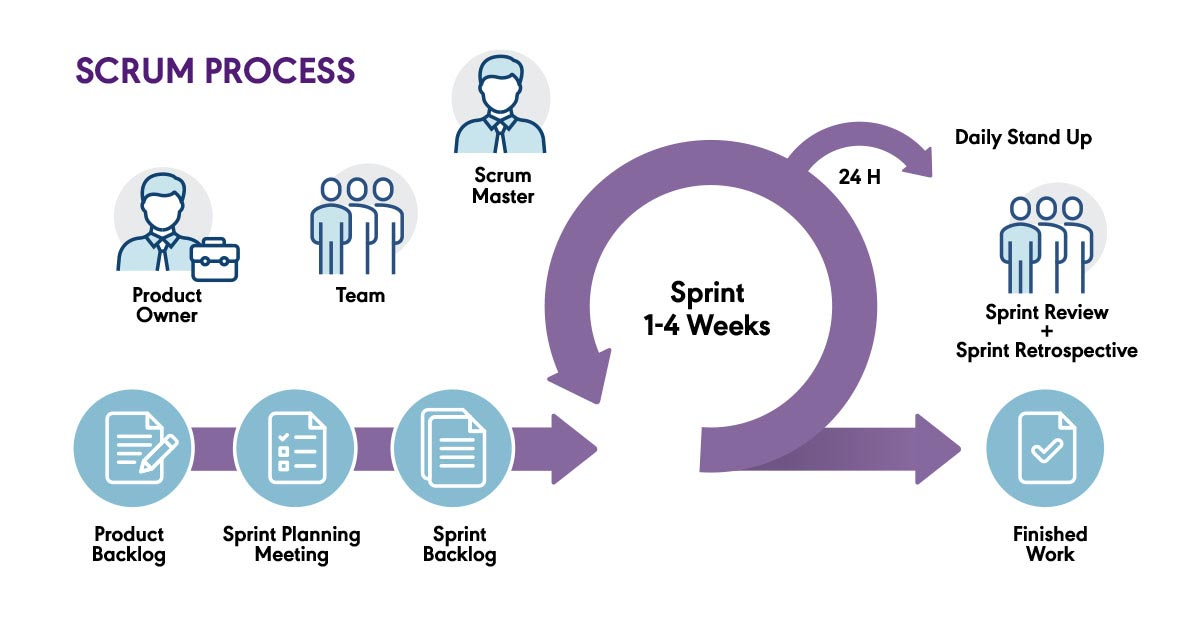
\includegraphics[width=0.7\textwidth]{src/assets/chapters/blog-scrum-process-opt.jpg}
    \caption{The Scrum Framework}
    \label{fig:Scrum_Framework_image}
\end{figure}




\subsubsection*{I.6.1.1 Members of a Scrum Team}
\addcontentsline{toc}{subsubsection}{\hspace{1.5em}I.6.1.1 Members of a Scrum Team}

At the core of Scrum lies a compact team configuration. This team is composed of a Scrum Master, a Product Owner, and Developers. The structure of a Scrum Team is flat, with no subdivisions or levels of authority. This unified group of professionals dedicates its efforts to achieving a single aim the Product Goal with collective focus and collaboration.

\textbf{Developers:} These are the individuals within the Scrum Team dedicated to delivering a functional segment of the product in every Sprint.

\textbf{Product Owner:} This role is filled by a single individual who represents the interests of various stakeholders in the Product Backlog. The Product Owner is responsible for effectively managing the Product Backlog and maximizing the value produced by the Scrum Team.

\textbf{Scrum Master:} Possesses a thorough understanding of the team’s tasks and guides the team in enhancing their workflow and transparency. Acting as the primary facilitator, the Scrum Master arranges the necessary resources, both people and logistical, for conducting sprint planning, daily stand-ups, sprint reviews, and sprint retrospectives.



\begin{figure}[H]
    \centering
    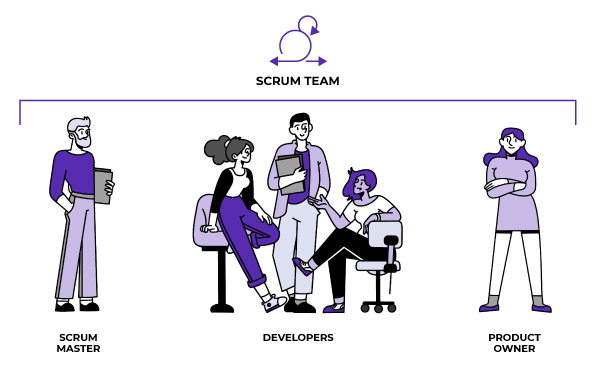
\includegraphics[width=0.7\textwidth]{src/assets/chapters/scrumTeam.jpg}
    \caption{The Scrum Team}
    \label{fig:Scrum_Team_image}
\end{figure}




\subsubsection*{I.6.1.2 Scrum events}
\addcontentsline{toc}{subsubsection}{\hspace{1.5em}I.6.1.2  Scrum events}

The Sprint acts as the framework for all Scrum activities, with each event within Scrum providing a structured opportunity to review and refine the Scrum artifacts. These events are deliberately designed to foster the necessary openness.

\textbf{The Sprint:} Sprints form the core rhythm of Scrum, transforming concepts into tangible value. These are fixed-duration events, capped at one month or less, to maintain regularity. The commencement of a new Sprint immediately follows the end of the preceding one.

\textbf{Sprint Planning:} This session involves the entire development team and focuses on delineating the tasks for the upcoming Sprint. Selections from the product backlog, specifically user stories that align with Sprint’s goal, are chosen and deemed achievable by the team.

\textbf{Daily Scrum:} This is a brief, 15-minute check-in for the development team, occurring every day of the Sprint, aimed at evaluating progress towards the Sprint Goal and adjusting the Sprint Backlog as required.

\textbf{Sprint Review:} Conducted at the end of each Sprint, this meeting assesses the Sprint’s output and identifies adjustments for the future. The Scrum Team showcases their work to key stakeholders, and discussions revolve around progress towards the Product Goal.

\textbf{Sprint Retrospective:} This meeting focuses on enhancing quality and efficiency. The Scrum Team pinpoints the most significant changes needed to boost their effectiveness, with an emphasis on implementing these improvements promptly.

\subsubsection*{I.6.1.3  Scrum artifacts}
\addcontentsline{toc}{subsubsection}{\hspace{1.5em}I.6.1.3 Scrum artifacts}

Scrum artifacts embody either work or value, created to ensure the transparency of crucial information is maximized. This allows all stakeholders examining these artifacts to have a consistent understanding of making adjustments.

\textbf{Product Backlog:} This is the comprehensive list of tasks to be completed, encompassing features, improvements, and fixes that serve as inputs for the Sprint Backlog. Managed actively by the Product Owner, the Product Backlog is continually updated, reprioritized, and refined to reflect changes in project needs or solutions.

\textbf{Sprint Backlog:} Comprised of items, user stories, or fixes chosen by the development team for the current Sprint. The Sprint Backlog is adaptable, allowing for adjustments throughout the Sprint to better meet the Sprint’s objectives without losing sight of the overall goal.

\textbf{Increment:} Represents a tangible step towards achieving the Product Goal. Each Increment builds upon previous ones, ensuring compatibility and comprehensive functionality. An Increment must be in a usable condition to deliver real value.

\subsubsection*{I.6.2 Kanban}
\addcontentsline{toc}{subsubsection}{I.6.2 Kanban}
Kanban, originating from Japanese words meaning "visual sign" or "card," serves as a visual framework for embracing Agile methodologies. It encourages incremental changes within the current system. Core principles of Kanban involve visualizing the workflow, setting limits on work in progress, optimizing and refining the flow, explicitly defining policies, and fostering continuous improvement .


\begin{figure}[H]
    \centering
    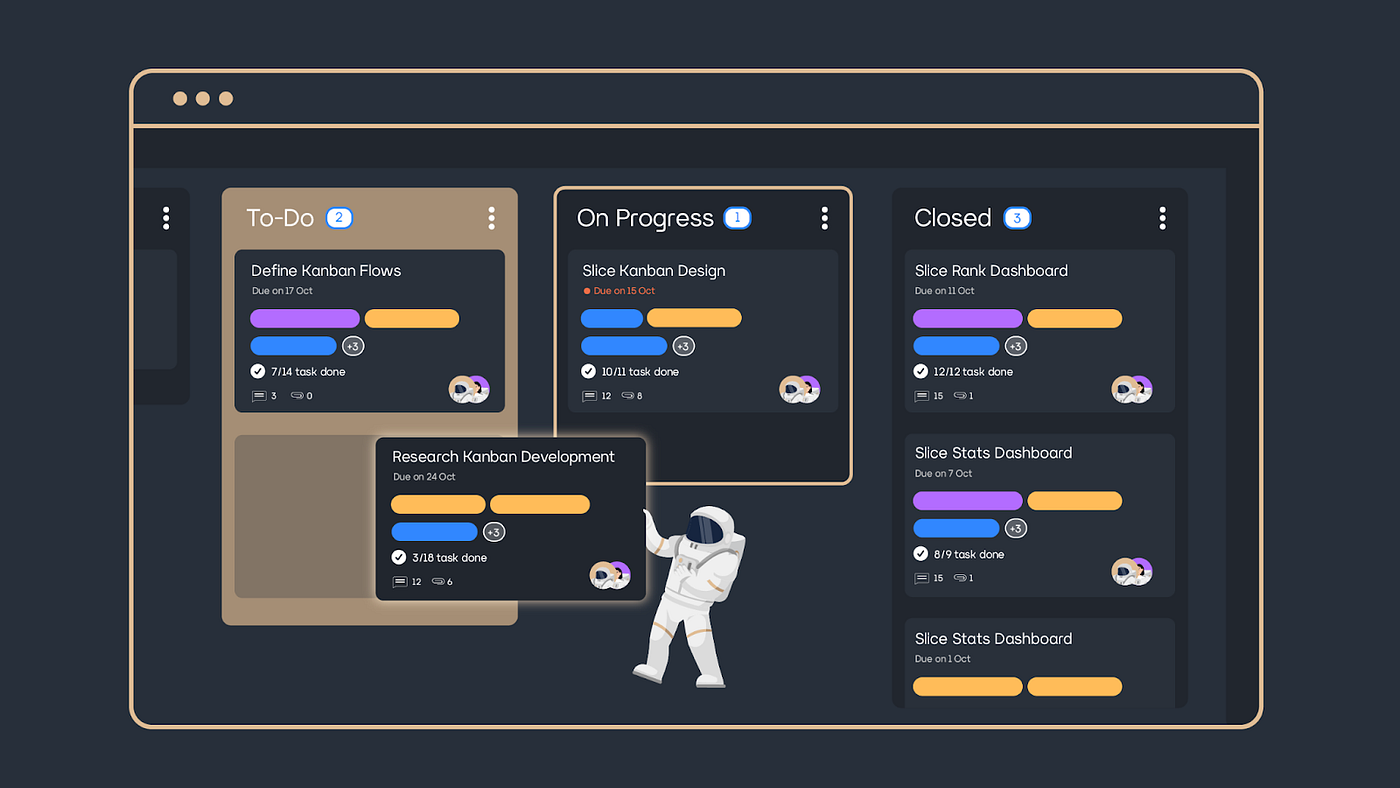
\includegraphics[width=0.7\textwidth]{src/assets/chapters/kanban.png}
    \caption{The illustration of columns in Sequence Stats Kanban}
    \label{fig:Kanban_Framework_image}
\end{figure}

Kanban operates as a continuous process, distinguished from Scrum's sprints, and emphasizes seamless workflow and continuous improvement. Here are key points about Kanban:

\begin{itemize}
    \item Workflow: Work items are pulled directly from the Product Backlog, ensuring a seamless flow.
    \item Work in Progress (WIP) Limit: Each column on the Kanban board has a strict limit for WIP to maintain optimal flow.
    \item Dispatching Indicators: Empty spots in columns signal the need to pull items from the preceding column.
    \item Daily Stand-up: Kanban prioritizes efficiency in daily stand-up meetings, with optional participation.
    \item Delivery: Products are delivered promptly upon completion, reflecting Kanban's emphasis on continuous delivery.
    \item Demo and Retrospective: Continuous revisions and retrospectives drive ongoing improvement in process efficiency and deliverable quality.
\end{itemize}


\subsubsection*{I.6.3 Scrumban}
\addcontentsline{toc}{subsubsection}{I.6.3 Scrumban}

Scrumban is a hybrid Agile methodology that combines elements of Scrum and Kanban. Here are key points about Scrumban:

\begin{itemize}
    \item Hybrid Methodology: Scrumban blends the flexibility of Kanban with the structure of Scrum to optimize workflow.
    \item Continuous Improvement: Like Kanban, Scrumban emphasizes continuous improvement through visualizing workflow and limiting Work in Progress (WIP).
    \item Iterative Approach: Scrumban maintains Scrum's iterative approach, allowing for regular review and adaptation of processes.
    \item Adaptive Planning: Scrumban enables adaptive planning, allowing teams to adjust priorities and resources based on changing requirements.
    \item Lean Principles: Scrumban incorporates Lean principles, such as eliminating waste and maximizing value delivery, to streamline processes.
\end{itemize}


\begin{figure}[H]
    \centering
    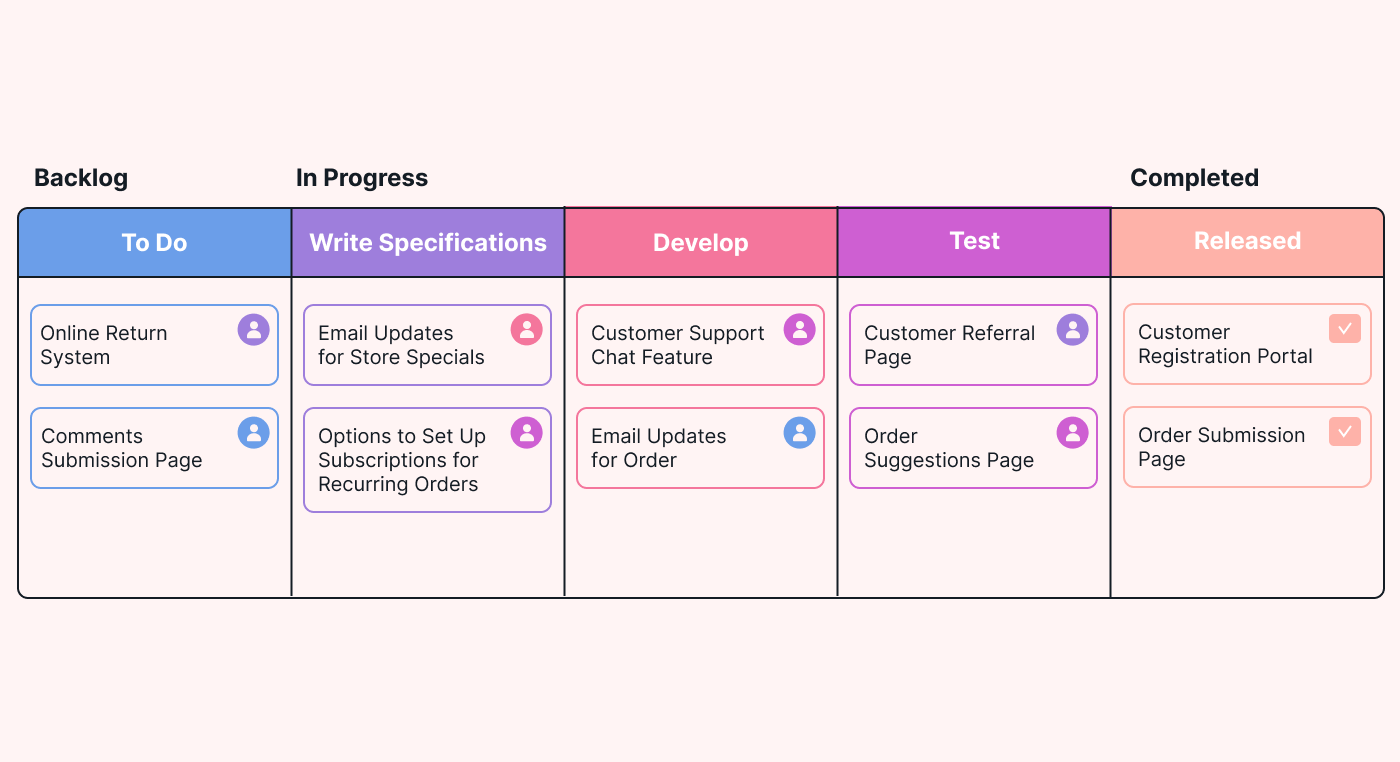
\includegraphics[width=0.7\textwidth]{src/assets/chapters/Scrumban.png}
    \caption{The Scrumban board}
    \label{fig:Scrumban_image}
\end{figure}


\subsubsection*{I.6.4 Evaluation of PM frameworks}
\addcontentsline{toc}{subsubsection}{I.6.4 Evaluation of PM frameworks}
To summarize, Scrum stands out as a highly effective Agile framework due to its structured approach and emphasis on iterative development. Unlike traditional project management methodologies, Scrum encourages regular collaboration and communication among team members, fostering a cohesive and efficient working environment. The use of fixed-length sprints allows for predictable delivery timelines and frequent feedback cycles, ensuring that any issues or changes can be addressed promptly. Additionally, Scrum's clear roles and responsibilities, including the Product Owner, Scrum Master, and Development Team, provide clarity and accountability throughout the project lifecycle. By prioritizing customer satisfaction and adapting to changing requirements through continuous improvement, Scrum enables teams to deliver high-quality products efficiently and effectively.

\subsubsection*{I.6.5 Choice of development methodology}
\addcontentsline{toc}{subsubsection}{I.6.5 Choice of development methodology}


Scrum has been chosen as the preferred development methodology for the following reasons:

\begin{itemize}
    \item Structured Approach: Scrum offers a structured framework that ensures clear roles, responsibilities, and processes throughout the development lifecycle.
    \item Iterative Development: Scrum's iterative approach allows for regular feedback and adaptation, resulting in a more flexible and responsive development process.
    \item Predictable Delivery: The use of fixed-length sprints in Scrum provides predictability in delivery timelines, enabling stakeholders to plan effectively.
    \item Collaboration and Communication: Scrum promotes collaboration and communication among team members, fostering a cohesive working environment and enhancing productivity.
    \item Continuous Improvement: Scrum emphasizes continuous improvement through regular retrospectives, enabling teams to identify and address areas for enhancement.
\end{itemize}

\subsection*{Conclusion}
\addcontentsline{toc}{subsection}{Conclusion}

In conclusion, this chapter began with an introduction to the host organization, followed by a detailed assessment of the identified problems and their associated challenges. We then proceeded to evaluate the competitive landscape to understand the key issues we aim to address. Lastly, we described our team’s adoption of an agile methodology, emphasizing its role in enhancing flexibility and collaboration. The upcoming chapter will delve into Sprint 0, marking the commencement of the project. This phase involves establishing objectives and laying out the roadmap for subsequent sprints.
